\chapter{Hidden Markov Model design}

%This is what I did to test and confirm my hypothesis.


%You may want to split this chapter into sub chapters depending on your design. I suggest you change
%the title to something more specific to your project.

%This is where you describe your design process in detail, from component/device selection to actual
%design implementation, to how you tested your system. Remember detail is important in technical
%writing. Do not just write I used a computer give the computer specifications or the oscilloscopes part
%number. Describe the system in enough detail so that someone else can replicate your design as well
%as your testing methodology.

%If you use or design code for your system, represent it as flow diagrams in text.

This section focuses on the design of the HMM used to test the hyphotheses postulated above.

\section{Description of available dataset}

The available dataset was acquired from a moving dog using Inertia Measurement Units. 
Two inertial measurements units (IMU) were straped to the front and back of a dog. Each unit has an accelarometer, a gyroscope and a magnetometer. The dataset contains calibrated measurements of a dog running, walking, and trotting then walking; together with the footfalls. The footfall is represented by a binary value that indicates the state of the dog's leg: if it is on or above the ground, at a particular instant in its gait sequence. More specifically, the value 0 means leg up and the value 1 means leg down.
The four variables representing the footfalls effectively constitute the ground truth, informing us about the state in which the dog is, at a given time in its movement.

The dataset can be retrieved from nine different matlab files. Each file contains twenty four matlab variables. The variables of interest are listed in the table \ref{tab:dataset}. 

\begin{table}[h!] 
	\centering
	\begin{tabular}{ |c|c|c|c| } 
		
		\hline
		\multicolumn{4}{| c |} {Observations}\\
		\hline
		
	   	 Body part & Accelerometer & Gyroscope & Magnetometer \\ 
		\hline
 
		\multirow{3}{4em}{Front}  & accFrontX & FrontPitch & magFront\_cal \\
		
	  		 
		 	  & accFrontY & FrontRoll & magFront\_cal2\\
		      & accFrontZ & FrontYaw & magFront\_cal3\\
		      \hline
		
		\multirow{3}{5em|}{Back} & accBackX & BackPitch & magBack\_cal\\ 
		      & accBackY & BackRoll & magBack\_cal2\\
		      & accBackZ & BackYaw & magBack\_cal3\\
    \hline

	\end{tabular}
	\caption{IMU measurements and footfall variables in dataset}
	\label{tab:dataset}
\end{table}

The observations are continous and the statistical property are assumed to be stationary, i.e, the do not vary over time. In this sta
\subsubsection{stationary: statistical property do not vary over time or non-stationary: properties vary over time}

\subsubsection{pure or corrupted?}

\subsection{Quadrupede Gait sequence modelling}
One of the objectives of this project is to effectively model the gait sequence dynamic of the dog from IMU measurements using HMM.
Based on the fact that quadrupedes achieve inverted pendulum-like movements like humans, %%TODO: quote here
their gait dynamic can be modelled as a succession of latent states observed by measurements such as IMU data. The states representing the footfalls and the observations, the outputs of the accelerometer, gyroscope and the magnetometer. Similar to human gait mechanism, it is sound to assume that the current state of a quadrupede is conditionally dependent on its previous state. 
This inference combined with the statistical robustness of HMM makes it the best model candidate when the available dataset is not large enough.

\subsubsection{HMM model elements: states and observations properties}
The problem at hand requires 16 distinct state that make up the state vector S, shown in equation \ref{eq:state}
\begin{align} \label{eq:state}
S &= {S_i} = \{(LF, RF, LB, RB)\} = \{0000, 0001, 0010, ..., 1111\}.
\end{align}
\[|S| = N = 2^4 = 16\]
\[i = 1, 2, ..., 16\]

The 16 distinct states are derived from the combination of the four binary footfalls. In practice, the dataset may not reveal all the 16 states.

The stream of IMU measurement form the observation sequence. An observation instance is a row vector of K dimensions. The initial K value before any dimensionality reduction is 18, from the 18 IMU measurements.
Thus, an observation sequence O is a TxK matrix of continuous values as presented in \ref{eq:obs}. T is the total number of the successive measurements.
\begin{align} \label{eq:obs}
O &= \{Ok_t\} = O1_t, O2_t, ..., O18_t. \\
k &= 1, 2, ..., 18. \\
t &= 1, 2, ..., T.
\end{align}


\subsubsection{Splitting the 16-states HMM in two 4-states HHMs}
In order to simplify the problem, it was decided to split the the four legs in two sub-parts: two front legs and two back legs. This approach for spliting it was based on the two inverted-like movements for a quadrupede such as a dog has investigated in %%TODO: reference. 
As a result, the initial 16-states HMM becomes, two distinct 4-states HMMs. These two models may be combined to get back the holistic 16-states model. 
This design decision was motivated by the fact that it is a simpler task to dsicriminate between 4 distinct classses than 16 classes. From here onward, attention will be given to the 4-states HMM model.
 
\subsubsection{Transition between states}
%%TODO: fix the subscript
This design assumes that a dog can transition from one state to any other possible state. So, for any transtion from S\_{i} to S\_{j} both S\_{i} and S\_{j} may be any of the element of the state space 

\[S = \{S1, S2, S3, S4\}\].

For instance, if a dog has its left leg above ground and its right leg on ground, at time instance t, it may move to any of the 3 other possible positions or remain in the same state, in the next time instance, t + 1. 
This consideration yielded in an ergodic HMM where, all the transitions are possible. The graphical model of the simplified HMM is illustrated by figure \ref{fig:model}

\begin{figure}[ht]
	\centering
	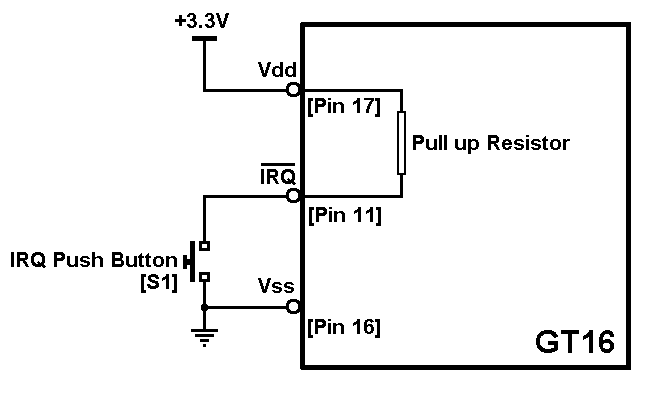
\includegraphics[width=0.7\textwidth]{model.png}
	\caption{Ergodic HMM graphical model showing the hidden states, observation, and transitions between states}
	\label{fig:model}
\end{figure}
%% TODO: Draw a simplified diagram of the 16 connected states with observations

\subsection{Data pre-processing}

\subsection{Model parameters estimation}
As a reminder, a continuous HMM model is completely specified by its initial state distribution: \(\pi\) transition matrix: A; the mean covariance matrices: \(\mu\), \(\Sigma\) which can be combined into \(\Phi\). If the observations are modelled with gaussian mixture distributions, one addition parameter is required for the initial mixture distribution: \(\beta\). The next sub-sections discuss how each parameters was estimated in this project.

\subsubsection{Transition matrix: A}
For each of the front and back 4-state HMM, the state transition matrix A, is a 4-by-4 matrix. Two different approaches were considered in the estimation of A. The two methods make use of the expectation maximisation algorithm %%TODO: Quote
but differ in the input arguments considered.

\begin{enumerate}
	%%TODO draw markov chain diagram
	\item Approach 1: Exploiting the available ground truth\\
	This approach takes advantage of the ground truth for a labelled dataset to reduce the HMM model to a Markov Chain. This is done by making the hypothetical observation sequence identical to the state sequence. Then, using approach used in discrete HMM, %%TODO: Quote
	the transition matrix can be estimated using maximum likelihood algorithm. %%TODO: Quote
	For each state, the pseudocount was set to the number of occurences of that state in the training data plus a constant value: \(PseudoA = |S_i| + C\). The additional constant C is to avoid having 0 in the transition matrix for states and transitions not reflected in the dataset. It can be chosen empirically.
	This method is very simple however, it has two limitations. It not only assumes that the number of states is known but also requires the training data to be labelled. Although, the dataset at hand satisfies the two constraints, the second approach which eliminates these possible setbacks, was also considered. \\\\\
	%%TODO: Quote [1] Durbin, R., S. Eddy, A. Krogh, and G. Mitchison. Biological Sequence Analysis. Cambridge, UK: Cambridge University Press, 1998.
	
	\item Approach 2: This method is the standard approach found in literature using expectation algorithm such as Welch-Baum algorithm. %%TODO: cite 
	%%TODO: site papers to support claim 
	and described in the literature review. %%TODO: cross-reference
\end{enumerate}


\subsubsection{Mean and covariance matrices: \(\mu\), \(\Sigma\) and \(\beta\)}
%%TODO: justify use of Gaussian with this:
\iffalse 
Gaussian
mixture models (GMMs) are powerful in modeling any
desired continuous distribution and are used for example in
speech processing successfully. Therefore, in this paper HMM
with GMMs as output density functions is trained and used
for human motion classification
\fi
The observations were modelled using mixture Gaussian distributions, characterised by a KxMxN mean matrix: \(\mu\) and a KxKxMxN co-variance matrix: \(\Sigma\).
where: \\ \(K = number \quad of \quad features, \quad M = mixture \quad number, \quad and \quad N = number \quad of \quad states\).
The observations were grouped K classes following based on the ground-truth represented by the state sequence.
The each group of observation was used as input to the EM algorithm to estimate the  \(\mu\) and \(\Sigma\).
In general, the optimal number of mixture, M is chosen empirically, in this project, it was estimated using akaike information criterion (AIC).
So, gaussian mixture models were built using EM algorithm while varying the M from 1 to K, the feature number.
Since AIC is a measure of information loss, the model with the minimum AIC best represents the dataset. The number of mixture M, is therefore set to the mixture number of this model.
This algorithm is outlined below.
\begin{lstlisting}[language=Matlab] 
function M = best_M(data, K)
	data = training_set
	AIC = zeros(1, K);
	models = cell(1, K);
	for m = 1:K
		model = gauss_mixture(data, m);
		AIC(m) = model.AIC;
	end
	[minAIC, minAIC_Idx] = min(AIC);
	M = minAIC_Idx;
end
\end{lstlisting} 

The mixture components were considered evenly distributed initially.
In order to avoid zero values in the covariance matrix, it was regularized with \(10^-10\).
The maximum number of iteration of the EM algorithm was empirically set to 1000.

\subsubsection{Inital state distribution: \(\pi\)}
The initial state distribution was estimated using the probability of occurence of each state in the training data sample.
Thus, \(\pi = \{\pi_i\} = \frac{|S_i|}{T} \)
\subsection{Dimension reduction}
\subsubsection{Optimal number of features}

\begin{figure}[ht!]
	\includegraphics{Figures/MCE}
	\caption{Misclassification error vs feature number using separability index and KNN}
	\label{fig:opt-dim}
\end{figure}

\subsubsection{Optimal PCA component number}
\begin{figure}[ht!]
	\includegraphics{Figures/best_PCA}
	\caption{Optimal PCA component number}
	\label{fig:opt-pca}
\end{figure}

\section{HMM implementation}
\subsection{Proving learning ability by increasing loglik for many iteration: check one of papers}